\documentclass[dvipsnames]{standalone}

\usepackage[english]{babel}
\usepackage[linesnumbered, ruled, vlined]{algorithm2e}

\usepackage{caption}

% to create listings

\usepackage{listings, lstautogobble}
\lstset{
  autogobble=true,
  frame=single,
}

\lstdefinelanguage{coq}[Objective]{Caml}{
  morekeywords={Structure, Definition, Inductive, list, return},
  sensitive=true
}

% to define font size

\usepackage{ulem}
\usepackage{moresize}
\usepackage{anyfontsize}

% to use tikz and its libraries

\usepackage{tikz-timing}
\usepackage{tikz}

\usetikzlibrary{backgrounds}
\usetikzlibrary{decorations.pathreplacing, positioning, calc, arrows, shapes, automata, petri, patterns}

% to use tikzmark, to place and refer to marks outside the current figure

% \tikzset{every picture/.style={remember picture}}

% styles for transitions

\tikzset{transition/.append style={fill=black!20, thick}}
\tikzset{transition/.append style={fill=black!20, thick}}

% styles for test and inhib arcs.

\tikzstyle{test}=[pre, *-]
\tikzstyle{inhib}=[pre, o-]

% to use colors

\usepackage{xcolor}

%%%%%%%%%%%%%%%%%%%%%%%%%%%%%%%%%%%%%%%%%%%%%%%%%%
%                  BEGIN DOCUMENT                %
%%%%%%%%%%%%%%%%%%%%%%%%%%%%%%%%%%%%%%%%%%%%%%%%%%

\begin{document}

\begin{tikzpicture}

  % 
  % 1ST PN
  % 
  
  \node (pn1) {
    \begin{tikzpicture}

      % PLACES AND TRANSITIONS
      
      \node[place,tokens=2] (p0) {};
      
      \node[transition] (t0) at ($(p0)-(0,1)$) {};
      
      \node[place] (p1) at ($(t0)-(0,1)$) {};

      \node[transition] (t1) at ($(p1)-(0,1)$) {};

      % LABELS

      \node (pzLabel) at ($(p0)-(.7,-.2)$) { $p_0$};
      \node[anchor=east] (tzLabel) at ($(t0.west)$) {
        \begin{tabular}{@{}c@{}}
          $t_0$ \\
          $[2,4]$ \\
          \textcolor{red}{${<}$2${>}$} \\
        \end{tabular}
      };
      \node (poLabel) at ($(p1)-(.7,0)$) { $p_1$};
      \node (tzLabel) at ($(t1)-(.5,.2)$) { $t_1$};

      % ACTIONS, FUNCTIONS, CONDITIONS AND TIME ITVALS

      \node (a0) at ($(p0.east)+(.3,0)$) {\textcolor{Green}{$a_0$}};
      \node (a1) at ($(p1.east)+(.3,0)$) {\textcolor{red}{$a_1$}};

      \node[anchor=west] (c0) at ($(t0.east)$) {
        \begin{tabular}{@{}l@{}}
          \textcolor{Green}{$c_0$} \\
          \textcolor{red}{$f_0$} \\
        \end{tabular}
      };
      
      \node (c1) at ($(t1.east)+(.3,0)$) {\textcolor{red}{$c_1$}};
      
      % ARCS
      
      \draw (p0) edge[post] (t0);
      \draw (t0) edge[post] (p1);
      \draw (t1) edge[pre] (p1);
      \draw ($(t1.west)$) edge[bend left=90,post] ($(p0.west)$);
    \end{tikzpicture}
  };

  \node[anchor=north, draw, circle, inner sep=1pt] at ($(pn1.south)$) {1};  

  % 
  % 2ND PN
  % 
  
  \node (pn2) at ($(pn1.east)+(2,0)$) {
    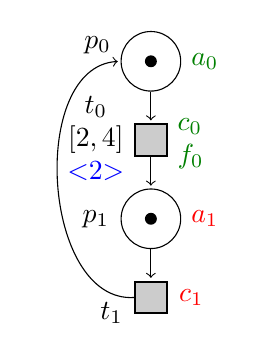
\begin{tikzpicture}

      % PLACES AND TRANSITIONS
      
      \node[place,tokens=1] (p02) {};      
      \node[transition] (t02) at ($(p02)-(0,1)$) {};
      \node[place,tokens=1] (p1) at ($(t02)-(0,1)$) {};
      \node[transition] (t1) at ($(p1)-(0,1)$) {};

      % LABELS

      \node[anchor=east] (pzLabel) at ($(p02.west)+(0,.2)$) {$p_0$};
      \node[anchor=east] (tzLabel) at ($(t02.west)$) {
        \begin{tabular}{@{}c@{}}
          $t_0$ \\
          $[2,4]$ \\
          \textcolor{blue}{${<}$2${>}$} \\
        \end{tabular}
      };
      \node (poLabel) at ($(p1)-(.7,0)$) { $p_1$};
      \node (tzLabel) at ($(t1)-(.5,.2)$) { $t_1$};

      % ACTIONS, FUNCTIONS, CONDITIONS AND TIME ITVALS

      \node (a0) at ($(p02.east)+(.3,0)$) {\textcolor{Green}{$a_0$}};
      \node (a1) at ($(p1.east)+(.3,0)$) {\textcolor{red}{$a_1$}};

      \node[anchor=west] (c0) at ($(t02.east)$) {
        \begin{tabular}{@{}l@{}}
          \textcolor{Green}{$c_0$} \\
          \textcolor{Green}{$f_0$} \\
        \end{tabular}
      };
      
      \node (c1) at ($(t1.east)+(.3,0)$) {\textcolor{red}{$c_1$}};
      
      % ARCS
      
      \draw (p02) edge[post] (t02);
      \draw (t02) edge[post] (p1);
      \draw (t1) edge[pre] (p1);
      \draw ($(t1.west)$) edge[bend left=90,post] ($(p02.west)$);
    \end{tikzpicture}
  };

  \node[anchor=north, draw, circle, inner sep=1pt] at ($(pn2.south)$) {2};  

  % 
  % 3RD PN
  % 

  \node (pn3) at ($(pn2.east)+(2,0)$) {
    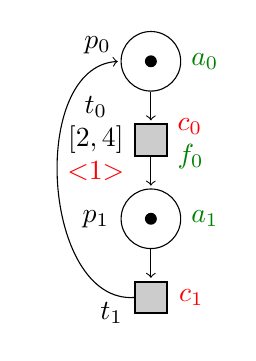
\begin{tikzpicture}

      % PLACES AND TRANSITIONS
      
      \node[place,tokens=1] (p02) {};      
      \node[transition] (t02) at ($(p02)-(0,1)$) {};
      \node[place,tokens=1] (p1) at ($(t02)-(0,1)$) {};
      \node[transition] (t1) at ($(p1)-(0,1)$) {};

      % LABELS

      \node[anchor=east] (pzLabel) at ($(p02.west)+(0,.2)$) {$p_0$};
      \node[anchor=east] (tzLabel) at ($(t02.west)$) {
        \begin{tabular}{@{}c@{}}
          $t_0$ \\
          $[2,4]$ \\
          \textcolor{red}{${<}$1${>}$} \\
        \end{tabular}
      };
      \node (poLabel) at ($(p1)-(.7,0)$) { $p_1$};
      \node (tzLabel) at ($(t1)-(.5,.2)$) { $t_1$};

      % ACTIONS, FUNCTIONS, CONDITIONS AND TIME ITVALS

      \node (a0) at ($(p02.east)+(.3,0)$) {\textcolor{Green}{$a_0$}};
      \node (a1) at ($(p1.east)+(.3,0)$) {\textcolor{Green}{$a_1$}};

      \node[anchor=west] (c0) at ($(t02.east)$) {
        \begin{tabular}{@{}l@{}}
          \textcolor{red}{$c_0$} \\
          \textcolor{Green}{$f_0$} \\
        \end{tabular}
      };
      
      \node (c1) at ($(t1.east)+(.3,0)$) {\textcolor{red}{$c_1$}};
      
      % ARCS
      
      \draw (p02) edge[post] (t02);
      \draw (t02) edge[post] (p1);
      \draw (t1) edge[pre] (p1);
      \draw ($(t1.west)$) edge[bend left=90,post] ($(p02.west)$);
    \end{tikzpicture}
  };

  \node[anchor=north, draw, circle, inner sep=1pt] at ($(pn3.south)$) {3};  

  %
  % EDGES between PNs
  % 

  \draw ($(pn1.west)-(.6,0)$) edge[->,double, line width=1pt] node[above,midway]{\Large$\downarrow$} ($(pn1.west)+(.2,0)$);
  \draw ($(pn1.east)-(.1,0)$) edge[->,double, line width=1pt] node[above,midway]{\Large$\uparrow$} ($(pn2.west)+(.1,0)$);
  \draw ($(pn2.east)-(.1,0)$) edge[->,double, line width=1pt] node[above,midway]{\Large$\downarrow$} ($(pn3.west)+(.1,0)$);
  \draw ($(pn3.east)-(.1,0)$) edge[->,double, line width=1pt] node[above,midway]{\Large$\uparrow$} ($(pn3.east)+(.6,0)$);
  
  \node at ($(pn1.west)-(.9,0)$) {\dots};
  \node at ($(pn3.east)+(.9,0)$) {\dots};
\end{tikzpicture}

\end{document}